\seccion{Entrop\'ia como medida de incerteza}
\label{Sec:SZ:Entropia}

% ================================= Axiomas

\subseccion{Entrop\'ia de Shannon, propiedades}
\label{Ssec:SZ:DefinicionShannon}

Uno de los primeros trabajos tratando de formalizar la noci\'on de informaci\'on
de  una cadena  de s\'imbolos  es debido  a Ralph  Hartley~\cite{Har28}.   En su
papel,  Hartley  defini\'o  la   informaci\'on  de  una  secuencia  como  siendo
proporcional a su longitud.  M\'as  precisamente, para s\'imbolos de un alfabeto
de cardinal $\alpha$,  existen $\alpha^n$ cadenas distintas de  longitud $n$. Se
defini\'o la informaci\'on  de tales cadenas como siendo  $K n$ ($K$ dependiente
de  $\alpha$).    Para  ser  consistente,  dos  conjuntos   del  mismo  tama\~no
$\alpha_1^{n_1} =  \alpha_2^{n_2}$ deben llegar a la  misma informaci\'on, as\'i
que  la informaci\'on  de  Hartley es  definida  como $H  = \log\left(  \alpha^n
\right)$  donde la  base del  logaritmo es  arbitraria.  Dicho  de  otra manera,
tomando  un logaritmo  de  base 2,  esta  informaci\'on es  nada  m\'as que  los
n\'umeros de bits (0-1) necesarios  para codificar todas las cadenas de longitud
$n$  de s\'imbolos de  un alfabeto  de cardinal  $\alpha$.  La  informaci\'on de
Hartley  es  el equivalente  de  la entrop\'ia  de  Boltzmann  de la  mec\'anica
estad\'istica, la famosa  f\'ormula $S = k_B \log  W$~\cite{Bol96, Bol98, Jay65,
  Mer10, Mer18}.

Una debilidad del enfoque de Hartley es que considera impl\'icitamente que en un
mensaje, cada cadena de longitud dada  puede aparecer con la misma frecuencia, o
probabilidad   $1/\alpha^n$   (en   Boltzmann,   misma  probabilidad   de   cada
configuraci\'on),  siendo   la  informaci\'on   menos  el  logaritmo   de  estas
probabilidades.  Al  contrario, parece m\'as l\'ogico  considerar que secuencias
muy frecuentes  no llevan mucha  informaci\'on (se sabe que  aparecen), mientras
que las que  aparecen raramente llevan m\'as informaci\'on  (hay m\'as sorpresa,
m\'as incerteza  en observarlas).  Volviendo  a los s\'imbolos  elementales $x$,
vistos  como aleatorios  (o  valores, o  estados  que puede  tomar una  variable
aleatoria), la  (falta de)  informaci\'on o incerteza  va a  estar \'intimamente
vinculada a la probabilidad de aparici\'on de estos s\'imbolos $x$. Siguiendo la
idea de Hartley,  la informaci\'on elemental asociada al estado $x$  va a ser $-
\log p(x)$ donde $p(x)$ es la  probabilidad de aparici\'on de $x$.  Se define la
incerteza asociada a la variable  aleatoria como el promedio estad\'istico sobre
todos  los  estados posibles  $x$~\cite{Sha48,  ShaWea64}~\footnote{En la  misma
  \'epoca que Shannon, independientemente, medidades informacionales aparecieron
  en  c\'alculos de  capacidad  de canal  en  varios trabajos  como  los de  los
  ingenieros     franceses     Andr\'e     Clavier~\cite{Cla48}    o     Jacques
  Laplume~\cite{Lap48},   o    en   el   libro    del   estadounidense   Norbert
  Wiener~\cite[Cap.~III]{Wie48}  entre  varios  otros (ver~\cite[y  Ref.]{Ver98,
    Lun02, RioMag14, FlaRio16, RioFla17, Che17}).}.
%
\begin{definicion}[Entrop\'ia de Shannon]
\label{Def:SZ:Shannon}
%
  Sea  $X$  una  variable  aleatoria  definida  sobre  un  alfabeto  discreto  \
  $X(\Omega) = \X = \{ x_1 \, , \, \ldots \,  , \, x_\alpha \}$ \ de cardinal $\alpha = |\X|
  < + \infty$ finito. Sea $p_X$  la distribuci\'on de probabilidad de $X$, \ie $
  \forall \, x \in \X, \quad p_X(x) = P(X = x)$.  La entrop\'ia de Shannon de la
  variable $X$ est\'a definida por
  %
  \[
    H(p_X) = H(X) = - \sum_{x \in \X} p_X(x) \, \log p_X(x),
  \]
  %
  con la  convenci\'on \ $0 \log  0 = 0$ \  ($\displaystyle \lim_{t \to  0} \, t
  \log t = 0$).
\end{definicion}
%
\noindent La  base del logaritmo es  arbitraria; si es $\log_2$  el logaritmo de
base  2, $H$  est\'a en  unidades  binarias o  bits (se  encuentra tamb\'ien  la
denominaci\'on Shannons),  si se usa el  logaritmo natural $\ln$,  $H$ est\'a en
unidades naturales o nats, si es el de base 10, $H$ se da en d\'igitos decimales
o dits (se encuentra tamb\'ien la denominaci\'on bans o Hartleys).  {\it En este
  cap\'itulo,  se usar\'a  $H$ sin  especificar la  base del  logaritmo.   Si es
  necesario  que  tenga   una  base  $a$  dada,  se   denotar\'a  la  entrop\'ia
  correspondiente  $H_a$ y se  especificar\'a la  base del  logaritmo $\log_a$}.
Notar que $\log_a x = \frac{\log x}{\log a}$, dando
%
\[
H_a(X)  =  H_b(X)  \log_a b.
\]
%
En  lo  que  sigue, a\'un  que,  rigurosamente,  $H$  sea  una funci\'on  de  la
distribuci\'on  de  probabilidad $p_X$  y  no de  la  variable  $X$, se  usar\'a
indistintamente  tanto  la notaci\'on  $H(p_X)$  como  $H(X)$  seg\'un lo  m\'as
conveniente.  Adem\'as, $p_X$  podr\'a denotar indistintamente la distribuci\'on
de  probabilidad,  o  el  vector  de probabilidad  $p_X  \equiv  \begin{bmatrix}
  p_X(x_1) & \cdots & p_X(x_\alpha) \end{bmatrix}^t$.  En lo que sigue, de vez a
cuando, usaremos $p_i \equiv p_X(x_i)$ por simplificaci\'on de escritura.

$H$ es el equivalente de la entrop\'ia de Gibbs en mec\'anica estad\'istica.  La
letra  $H$  viene del  teorema-H  debido  a\ldots Ludwig  Boltzmann~\cite{Jay65,
  Mer10, Mer18}.

$H$ tiene propiedades notables que corresponden  a las que se puede exigir a una
medida de incerteza~\cite{Sha48, ShaWea64, CovTho06, Rio07, DemCov91, Joh04}.
%
\begin{propiedades}
\item\label{Prop:SZ:continuidad} {\it Continuidad:}  vista como una funci\'on de
  \ $\alpha$ \ variables  \ $p_i = p_X(x_i)$, \ $H$ \  es continua con respeto a
  los $p_i$.
%
\setcounter{PropPermutacion}{\value{enumi}}
\item\label{Prop:SZ:permutacion}   {\it  Invariance  bajo   una  permutaci\'on:}
  obviamente,  la  entrop\'ia  es  invariante  bajo  una  permutaci\'on  de  las
  probabilidades, \ie
  %
  \[
  \mbox{para   cualquiera   permutaci\'on   }   \sigma:   \X   \to   \X,   \quad
  H(p_{\sigma(X)})   =  H(p_X)   \quad  \mbox{con}   \quad   p_{\sigma(X)}(x)  =
  p_X(\sigma(x)),
  \]
  %
  lo que se  escribe tambi\'en $H(\sigma(X)) = H(X)$.   En particular, denotando
  $p_X^\downarrow$  el vector  de  probabilidades obtenido  a  partir de  $p_X$,
  clasificando  las  probabilidades en  orden  decreciente, $p_1^\downarrow  \ge
  p_2^\downarrow \ge  \cdots \ge p_\alpha^\downarrow$  donde $p_i^\downarrow$ es
  la $i$-\'esima componente de $p_X^\downarrow$,
  %
  \[
  H(p_X^\downarrow) = H(p_X).
  \]
%
\setcounter{PropBiyeccion}{\value{enumi}}
\item\label{Prop:SZ:biyeccion}   {\it  Invariance   bajo   una  transformaci\'on
    biyectiva:}  la entrop\'ia  es invariante  bajo  cualquiera transformaci\'on
  biyectiva, \ie
  %
  \[
  \mbox{para cualquiera  funci\'on biyectiva } g:  \X \to g(\X),  \quad H(g(X)) =
  H(X).
  \]
  %
  A  trav\'es  tal transformaci\'on  los  estados  cambian,  pero no  cambia  la
  distribuci\'on de probabilidad vinculada al alfabeto transformado.  Tomando el
  ejemplo de  un dado, la  incerteza vinculada al  dado no debe depender  de los
  s\'imbolos escritos sobre las caras, sean enteras o cualesquiera letras.
%
\item\label{Prop:SZ:positividad} {\it Positividad:} la entrop\'ia es acotada por
  debajo,
  %
  \[
  H(X) \ge 0,
  \]
  %
  con igualdad si y solamente si existe un $x_j \in \X$ tal que $p_X(x_j) = 1$ \
  y \ $p_X(x) = 0$ \ para \ $x \ne x_j$, \ie $p_X = \un_j$,
  %
  \[
  H(X)  =  0 \quad  \mbox{ssi}  \quad X  \mbox{  es  determinista.}
  \]
  %
  En  otras  palabras, cuando  $X$  no  es aleatoria,  \ie  $X  =  x_j$, no  hay
  incerteza, o  la observaci\'on  no lleva  informaci\'on (se sabe  lo que  va a
  salir, sin duda): $H = 0$.   La positividad es consecuencia de $p_X(x) \le 1$,
  dando $- p_X(x) \log p_X(x) \ge 0$.  Adem\'as, la suma de t\'erminos positivos
  vale cero  si y  solamente si  cada t\'ermino de  la suma  vale cero,  dando \
  $p_X(x) = 0$ \  o \ $p_X(x) = 1$. Se concluye  $p_X$ siendo una distribuci\'on
  de probabilidad, sumando a 1.
%
\setcounter{PropCotamaxima}{\value{enumi}}
\item\label{Prop:SZ:cotamaxima} {\it Maximalidad:}  la entrop\'ia es acotada por
  arriba,
  %
  \[
  H(X) \le \log \alpha,
  \]
  %
  con igualdad si y solamente si existe $X$ es uniforme sobre $\X$, \ie
  %
  \[
  H(X) =  \log \alpha \quad \mbox{ssi}  \quad \forall \,  x \in \X, \:  p_X(x) =
  \frac{1}{\alpha}.
  \]
  %
  En otras palabras, la incerteza  es m\'axima cuando cualquier estado $x$ puede
  aparecer con la misma probabilidad; cada observaci\'on lleva una informaci\'on
  importante sobre el  sistema que genera $X$.  La cota  m\'axima resuelta de la
  maximizaci\'on de $H$ sujeto a $\sum_x p_X(x) = 1$, es decir, con la t\'ecnica
  del  Lagrangiano para  tomar  en cuenta  el v\'inculo~\cite{Mil00,  CamMar09},
  notando $p_i = p_X(x_i)$, hay que minimizar  $\sum_i (- p_i \log p_i + \eta \,
  p_i)$ donde el factor de Lagrange  \ $\eta$ \ se determinar\'a para satisfacer
  el  v\'inculo.  Se  obtiene sencillamente  que $\log  p_i =  -\eta$,  dando la
  distribuci\'on  uniforma.\newline La  figura Fig.~\ref{Fig:SZ:EntropiaBinaria}
  representa la entrop\'ia de un sistema a dos estados, de probabilidades \ $p_X
  = \begin{bmatrix}  r & 1-r \end{bmatrix}^t$  \ (ley de  Bernoulli de parametro
  $r$), entrop\'ia a veces dicha  {\it entrop\'ia binaria}, en funci\'on de $r$.
  Esta figura  ilustra ambas cotas  ($r = 1$  o 1, $r  = \frac12$) as\'i  que la
  invariancia bajo una permutaci\'on ($h(r) = H(r,1-r) = H(1-r,r) = h(1-r)$).
  %
  \begin{figure}[h!]
  %
  \begin{center}\begin{tikzpicture}
\shorthandoff{>}
%
% Entropia binaria
\begin{scope}[xscale=3.5,yscale=2.5]
%
\draw[>=stealth,->] (-.05,0)--(1.15,0) node[right]{\small $r$};
\draw[>=stealth,->] (0,-.05)--(0,1.1) node[above]{\small $h(r)$};
\draw[thick,domain=.01:.99,samples=200] (0,0)-- plot (\x,{-\x*log2(\x)-(1-\x)*log2(1-\x)}) --(1,0);
\draw (0,0)--(0,-.02) node[below]{\small $0$};
\draw (1,0)--(1,-.02) node[below]{\small $1$};
\draw (0,1)--(-.02,1) node[left]{\small $\log 2$};
\end{scope}
\end{tikzpicture}\end{center}
  %
  \leyenda{Entrop\'ia binaria  (de una variable de Bernoulli)  $h(r) = H(r,1-r)$
    en funci\'on de $r \in [0 \; 1]$.}
  %
  \label{Fig:SZ:EntropiaBinaria}
  \end{figure}
%
\item\label{Prop:SZ:expansabilidad} {\it Expansibilidad:}  A\~nadir un estado de
  probabilidad 0 no cambia la entrop\'ia, \ie sean \ $X$ \ definido sobre \ $\X$
  \ y \ $\widetilde{X}$ \ sobre \ $\widetilde{X}$,
  %
  \[
  \widetilde{\X}  =  \X  \cup  \{  \widetilde{x}_0  \}  \quad  \mbox{con}  \quad
  p_{\widetilde{X}}(x)  =   p_X(x)  \quad  \mbox{si}  \quad  x   \in  \X,  \quad
  p_{\widetilde{X}}(\widetilde{x}_0)   =   0,   \qquad   \mbox{entonces}   \quad
  H(p_{\widetilde{X}}) = H(p_X).
  \]
  %
  Esta propiedad  es obvia, consecuencia de  $\displaystyle \lim_{t \to  0} \, t
  \log t = 0$.
%
\setcounter{PropRecursividad}{\value{enumi}}
\item\label{Prop:SZ:recursividad} {\it Recursividad:} Juntar dos estados baja la
  entrop\'ia de  una cantidad igual a  la entrop\'ia interna de  los dos estados
  por  la   probabilidad  de   ocurrencia  de  este   conjunto  de   estados,  y
  vice-versa. De la  invarianza de la entrop\'ia por  permutaci\'on, sin perdida
  de generalidad se  puede considerar que los estados que se  juntan son los dos
  \'ultimos, \ie sean \ $X$ \ definido  sobre \ $\X$ \ y \ $\breve{X}$ \ sobre
  \ $\breve{\X}$ \ tales que,
  %
  \[
  \left\{  \begin{array}{l}\breve{\X}  = \{  x_1  ,  \ldots  , x_{\alpha-2}  ,
      \breve{x}_{\alpha-1}\} \quad \mbox{con el estado interno} \quad
      \breve{x}_{\alpha-1}   =  \{   x_{\alpha-1} \,  , \,   x_\alpha  \},\\[2.5mm]
      p_{\breve{X}}(x_i) = p_X(x_i), \quad 1 \le i \le \alpha-1 \quad \mbox{y}
      \quad p_{\breve{X}}(\breve{x}_{\alpha-1}) = p_X(x_{\alpha-1}) +
      p(x_\alpha)  \quad  \mbox{distribuci\'on  sobre  }  \breve{\X}\\[2.5mm]
      \displaystyle   \breve{q}(x_j)  =   \frac{p_X(x_j)}{p_X(x_{\alpha-1})  +
        p_X(x_\alpha)},  \quad j =  \alpha-1, \alpha  \quad \mbox{distribuci\'on
        del estado interno}\end{array}\right.
  \]
  %
  entonces,
  %
  \[
  H(p_X)  =   H(p_{\breve{X}})  +  p_{\breve{X}}(\breve{x}_{\alpha-1})  \,
  H(\breve{q}),
  \]
  %
  lo que se escribe tambi\'en
  %
  \[
  H(p_1,\ldots,p_\alpha)  =  H(p_1,\ldots,p_{\alpha-2},p_{\alpha-1}+p_\alpha)  +
  \left(             p_{\alpha-1}+p_\alpha            \right)            H\left(
    \frac{p_{\alpha-1}}{p_{\alpha-1}+p_\alpha}                                  ,
    \frac{p_\alpha}{p_{\alpha-1}+p_\alpha}\right).
  \]
  %
  Esta relaci\'on  viene de $a \log  a + b  \log b = (a+b)  \left( \frac{a}{a+b}
    \log\left(  \frac{a}{a+b} \right)  + \frac{b}{a+b}  \log\left( \frac{a}{a+b}
    \right)   -   \log(  a   +   b  )\right)$   es   ilustrada   en  la   figura
  Fig.~\ref{Fig:SZ:Recursividad}.\newline
  %
  \begin{figure}[h!]
  %
  \begin{center} %\hskip 2.5cm
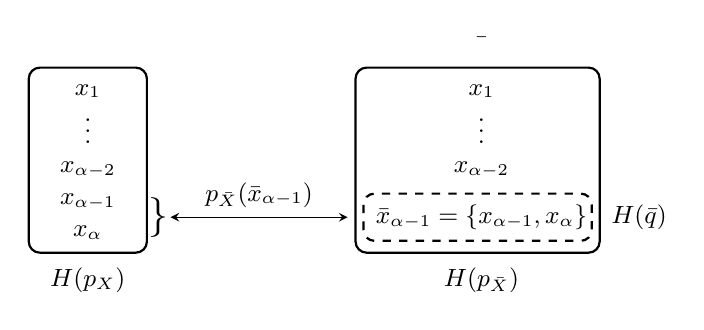
\begin{tikzpicture}
\shorthandoff{>}
%
% Ensemble \X
\draw(0,3) node{\small $\X$};
\draw(0,2.4) node{\small $x_1$};
\draw(0,2) node{\small $\vdots$};
\draw(0,1.4) node{\small $x_{\alpha-2}$};
\draw(0,1) node{\small $x_{\alpha-1}$};
\draw(0,.6) node{\small $x_{\alpha}$};
\draw(0,0) node{\small $H(p_X)$};
\draw[thick,rounded corners] (-.75,.35) rectangle (.75,2.7);
%
% Ensemble \bar{\X}
%
\draw(5,3) node{\small $\bar{\X}$};
\draw(5,2.4) node{\small $x_1$};
\draw(5,2) node{\small $\vdots$};
\draw(5,1.4) node{\small $x_{\alpha-2}$};
\draw(5,.8) node{\small $\bar{x}_{\alpha-1} = \{ x_{\alpha-1} , x_\alpha\}$};
\draw(5,0) node{\small $H(p_{\bar{X}})$};
\draw(7,.8) node{\small $H(\bar{q})$};
\draw[dashed,thick,rounded corners] (3.5,.5) rectangle (6.4,1.1);
\draw[thick,rounded corners] (3.4,.35) rectangle (6.5,2.7);
%
% juntando 2 estados VER PROBLEMA CON LA FLECHA
\draw(.9,.8) node{\Large $\}$};
\draw[>=stealth,<->] (1.05,.8)--(3.3,.8);
\draw (2.175,.8) node[above]{\small $p_{\bar{X}}(\bar{x}_{\alpha-1})$};
\end{tikzpicture} \end{center}
  %
  \leyenda{Ilustraci\'on de  la propiedad  de recursividad, que  cuantifica como
    decrece  la  entrop\'ia  en  un  conjunto  cuando  se  juntan  dos  estados,
    relacionando   la  entrop\'ia   total,  la   entrop\'ia  despu\'es   del  la
    agrupaci\'on y la entrop\'ia interna a los dos estados juntados.}
  %
  \label{Fig:SZ:Recursividad}
  \end{figure}
%
\setcounter{PropConcavidad}{\value{enumi}}
\item\label{Prop:SZ:concavidad}  {\it Concavidad:}  la  entrop\'ia es  c\'oncava
  ($-H$         es         convexa,        ver         Def.~\ref{Def:MP:convexa}
  pagina~\pageref{Def:MP:convexa}), en  el sentido de  que la entrop\'ia  de una
  combinaci\'on convexa de distribuciones  (mezcla) de probabilidades es siempre
  mayor o igual a la combinaci\'on convexa de entrop\'ias:
  %
  \[
  \forall \:  \{ \pi_i \}_{i=1}^n, \quad  0 \le \pi_i \le  1, \quad \sum_{i=1}^n
  \pi_i  = 1  \quad \mbox{and  cualquier  conjunto de  distribuciones} \quad  \{
  p_{(i)} \}_{i=1}^n,
  \]
  %
  \[
  H\left( \sum_{i=1}^n \pi_i \, p_{(i)} \right) \ge \sum_{i=1}^n \pi_i H(p_{(i)}).
  \]
  %
  Esta relaci\'on es conocida tambi\'en como desigualdad de Jensen~\cite{Jen06}.
  Es una consecuencia directa de la  convexidad de la funci\'on $\phi: t \mapsto
  t \log  t$, como ilustrado en la  figura Fig.~\ref{Fig:SZ:Concavidad}-(a).  La
  figura  Fig.~\ref{Fig:SZ:Concavidad}-(b)  ilustra como  se  puede obtener  una
  mezcla  de distribuciones  de dos  probabilidad $p_{(1)}$  (dado  izquierda) y
  $p_{(2)}$ (dado  derecho) haciendo  una elecci\'on aleatoria  a partir  de una
  moneda en  este ejemplo (probabilidad  $\pi_1 = 1  - \pi_2$ de elegir  el dado
  izquierda).\newline
  %
  \begin{figure}[h!]
  %
  \begin{center} \begin{tikzpicture}
\shorthandoff{>}
%
% Concavidad de - u log u
\begin{scope}[xscale=3,yscale=2.5]
\pgfmathsetmacro{\u}{.2};
\pgfmathsetmacro{\v}{1.25};
\pgfmathsetmacro{\l}{.7};
%
\draw[>=stealth,->] (-.5,0)--(1.6,0) node[right]{\small $t$};
\draw[>=stealth,->] (0,-.7)--(0,{1.5*log2(1.5)}) node[above]{\small $\phi(t) = t \log t$};
\draw[thick,domain=.005:1.5,samples=200] (0,0)-- plot (\x,{\x*log2(\x)});
\draw[dashed] (\u,{\u*log2(\u)})--(\v,{\v*log2(\v)});
\draw (\u,0)--(\u,-.05) node[below]{\small $t_1$};
\draw (\v,0)--(\v,-.05) node[below]{\small $t_2$};
%
\draw[dashed] ({\l*\u+(1-\l)*\v},.05) node[above]{\small $\pi_1 t_1 + \pi_2 t_2$}
--({\l*\u+(1-\l)*\v},{(\l*\u+(1-\l)*\v)*log2(\l*\u+(1-\l)*\v)});
%
% l phi(u) + (1-l) phi(v)
\draw[dotted]
({\l*\u+(1-\l)*\v},{\l*\u*log2(\u)+(1-\l)*\v*log2(\v)})--(-.05,{\l*\u*log2(\u)+(1-\l)*\v*log2(\v)})
node[left]{\small $\pi_1 \phi(t_1) + \pi_2 \phi(t_2)$};
%
% phi(l u + (1-l) v)
\draw[dotted]
({\l*\u+(1-\l)*\v},{(\l*\u+(1-\l)*\v)*log2(\l*\u+(1-\l)*\v)})--
(-.05,{(\l*\u+(1-\l)*\v)*log2(\l*\u+(1-\l)*\v)})
node[left]{\small $\phi(\pi_1 t_1 + \pi_2 t_2)$};
\end{scope}
%
%
% Concavidad / mezcla
\begin{scope}[xshift=8.5cm]
\draw(0,1.25) node{\includegraphics[width=3cm]{TIKZ_SZ/DosDados}};
\draw(-.5,2.5) node{\small $p_1$};
\draw(1,2) node{\small $p_2$};
\draw(2.7,1) node{\small $\pi_1 p_1 + \pi_2 p_2$};
\draw(-.25,-1) node{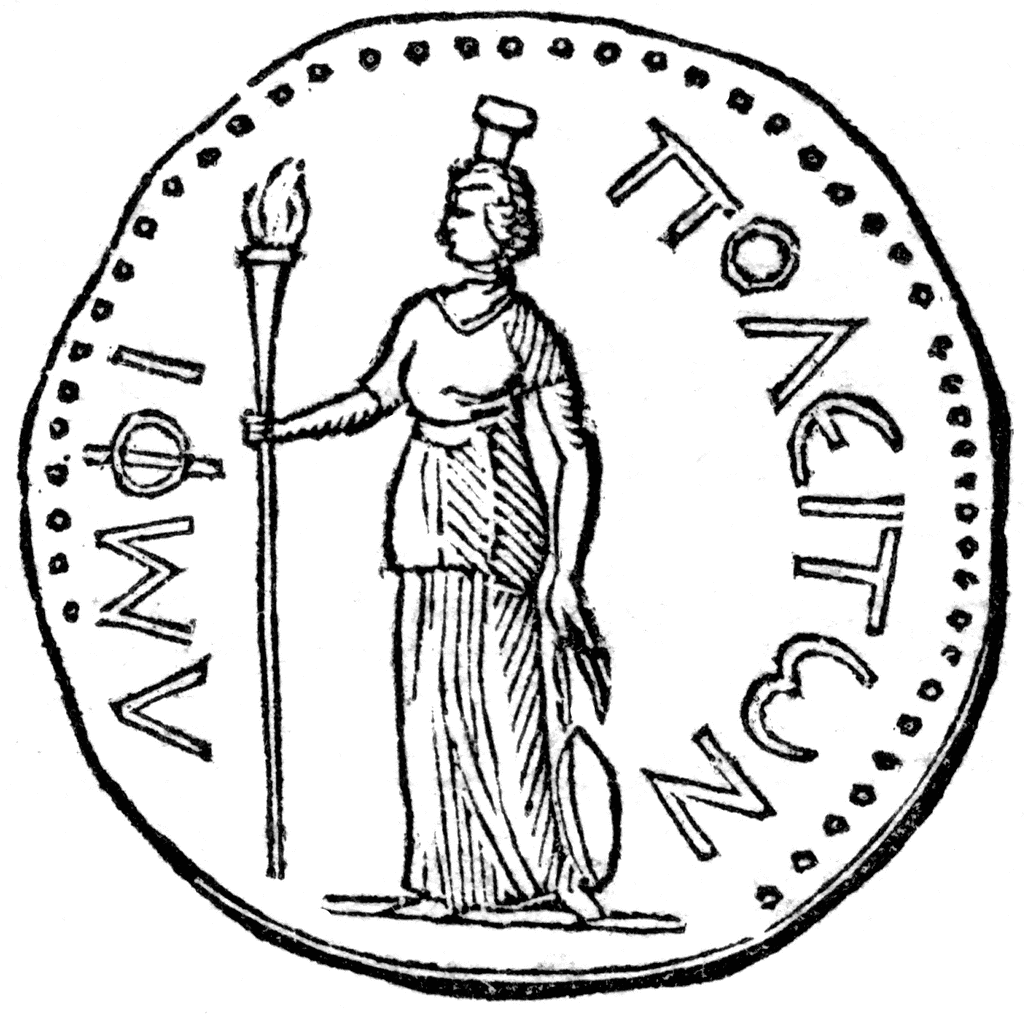
\includegraphics[width=1cm]{TIKZ_SZ/Moneda}};
\draw[>=stealth,->,thick] (-.3,-.35)--(-.75,.45);
\draw (-.525,0) node[left]{\small $\pi_1$};
\draw[>=stealth,->,thick] (-.2,-.35)--(.3,.45);
\draw (.05,0) node[right]{\small $\pi_2 = 1-\pi_1$};
\end{scope}
%
\draw (1.25,-2.25) node{(a)};
\draw (8.25,-2.25) node{(b)};
\end{tikzpicture} \end{center}
  %
  \leyenda{(a) $\phi(t)  = t \log t$ es  convexa: la curva es  siempre debajo de
    sus cuerdas; entonces, cada promedio de $\phi(t_1)$ y $\phi(t_2)$ estando en
    la cuerda juntando  estos puntos, queda arriba de la  funci\'on tomada en el
    promedio de $t_1$ y $t_2$.  Escribiendo eso para (m\'as de dos puntos) sobre
    los $\sum_i \pi_i \, p_{(i)}(x)$ y sumando sobre los $x$  da la desigualdad de
    Jensen.  (b) Ilustraci\'on de  una distribuci\'on de mezcla, ac\'a mezclando
    $p_{(1)}$ y $p_{(2)}$  a partir de una tercera  variable aleatoria (ac\'a de
    Bernoulli).}
  %
  \label{Fig:SZ:Concavidad}
  \end{figure}
%
\setcounter{PropSchurConcavidad}{\value{enumi}}
\item\label{Prop:SZ:Schurconcavidad}  {\it Schur-concavidad:}  como se  lo puede
  querrer, lo  m\'as ``concentrado'' es  una distribuci\'on de  probabilidad, lo
  menos hay  incerteza, y  entonces lo m\'as  peque\~no debe ser  la entrop\'ia.
  Esta propiedad intuitiva  se resuma a partir de  la noci\'on de mayorizaci\'on
  vista       en      la       definici\'on      Def.~\ref{Def:MP:Mayorizacion},
  pagina~\pageref{Def:MP:Mayorizacion}  (recuerdense  que  si  los  vectores  no
  tienen  el mismo  tama\~no, el  m\'as peque\~no  es completado  por  ceros; es
  equivalente a a\~nadir estados fictivos de probabilidad nula, lo que no cambia
  la entrop\'ia).
  %
%  \begin{definicion}[Mayorizaci\'on]\label{Def:SZ:Mayorizacion}
%    Un vector de  probabilidad (distribuci\'on) $p$ mayorizado por  un vector de
%    probabilidad (distribuci\'on) $q$, notado $p \prec q$, se define como:
%    %
%    \[
%    p  \prec   q  \qquad  \mbox{ssi}  \qquad   \sum_{i=1}^k  p_i^\downarrow  \le
%    \sum_{i=1}^k q_i^\downarrow, \quad  1 \le k < \alpha  \qquad \mbox{y} \qquad
%    \sum_{i=1}^\alpha p_i^\downarrow = \sum_{i=1}^\alpha q_i^\downarrow
%    \]
%    %
%    (las \'ultimas sumas siendo igual a 1).  Si los alfabetos de definici\'on de
%    \ $p$ \ y  \ $q$ \ son de tama\~nos diferentes, \  $\alpha$ \ es el tama\~no
%    lo m\'as  grande y  la distribuci\'on  sobre el alfabeto  lo m\'as  corto es
%    completada por  estados de probabilidad 0  (recordar que no va  a cambiar la
%    entrop\'ia).
%  \end{definicion}
  %
  La  Schur-concavidad  se  traduce  por  la  relaci\'on
  %
  \[
  p \prec  q \quad \Rightarrow  \quad H(p) \ge  H(q).
  \]
  %
  Fijense de  que las cotas  sobre $H$ pueden  ser vistas como  consecuencias de
  esta desigualdad: la  distribuci\'on cierta mayoriza cualquiera distribuci\'on
  y  cualquiera distribuci\'on  mayoriza la  distribuci\'on uniforme~\cite[p.~9,
  (6)-(8)]{MarOlk11}.  Adem\'as, de la Schur-concavidad se obtiene que
  %
  \[
  H\left( \begin{bmatrix}  \frac1\alpha & \cdots  & \frac1\alpha \end{bmatrix}^t
  \right) \quad \mbox{es una funci\'on creciente de } \alpha.
  \]
  %
  La prueba  de la  Schur-concavidad se  apoya sobre la  desigualdad de  Schur o
  Hardy-Littlewood-P\'olya    o     Karamata~\cite{Sch23,    HarLit29,    Kar32,
    HarLit52},~\cite[Cap.~3,                                 Prop.~C.1]{MarOlk11}
  o~\cite[Teorema~II.3.1]{Bha97}: $t \prec t' \: \Rightarrow \: \sum_i \phi(t_i)
  \le  \sum_i  \phi(t'_i)$  para  cualquiera  funci\'on  $\phi$  convexa.  Basta
  considerar $\phi(t) = t \log t$ para concluir.
\end{propiedades}
%
% Ver Schur-Ostrowski f  sym, Scur-convexe ssi (xi - xj)  (df/dx_i - df/dxj) \ge
% 0, 1 \le i \ne j \le alpha


En muchos  casos, uno tiene que  trabajar con varias  variables aleatorias. Para
simplificar las notaciones, consideramos  un par de variables \ $X$ \  y \ $Y$ \
definidas respectivamente sobre los alfabetos \ $\X$  \ y \ $\Y$ \ de cardinal \
$\alpha = |\X|$ \ y \ $\beta = |\Y|$.  Tal par de variables puede ser vista como
una  variable $(X,Y)$  definida sobre  el alfabeto  $\X \times  \Y$  de cardinal
$\alpha \beta$ tal que se  define naturalmente la entrop\'ia para esta variable;
tal entrop\'ia es llamada {\it entrop\'ia conjunta} de $X$ y $Y$:
%
\begin{definicion}[Entrop\'ia conjunta]
\label{Def:SZ:EntropiaConjunta}
%
  Sean \ $X$ \ e \ $Y$  \ dos variables aleatorias definidas sobre los alfabetos
  discretos \  $\X$ \ y \ $\Y$,  de cardinal \ $\alpha  = |\X| < +\infty$  \ y \
  $\beta  =  |\Y|   <  +\infty$  \  respectivamente.   Sea   \  $p_{X,Y}$  \  la
  distribuci\'on de probabilidad conjunta de \ $X$ \ e \ $Y$, \ \ie $ \forall \,
  (x,y) \in \X \times  \Y, \quad p_{X,Y}(x,y) = P( (X = x) \cap  (Y = y) )$.  La
  entrop\'ia conjunta de Shannon de las variables  \ $X$ \ e \ $Y$ \ es definida
  por
  %
  \[
  H(p_{X,Y}) =  H(X,Y) = -  \sum_{(x,y) \in \X  \times \Y} p_{X,Y}(x,y)  \, \log
  p_{X,Y}(x,y),
  \]
  %
  con la convenci\'on \ $0 \log 0 = 0$.
\end{definicion}

A partir de esta definici\'on,  aparecen otras propiedades importantes, sino que
fundamentales, de la entrop\'ia de Shannon.
%
\begin{propiedades}
\item\label{Prop:SZ:aditividad} {\it Aditividad:}  la entrop\'ia conjunta de dos
  variables aleatorias  \ $X$  \ e \  $Y$ \underline{independientes} se  suma, y
  rec\'iprocamente:
  %
  \[
  X \: \mbox{e} \: Y \: \mbox{independientes} \quad \Leftrightarrow \quad H(X,Y)
  =  H(X) +  H(Y).
  \]
  %
  Dicho de otra manera, para dos variables aleatorias, la incerteza global es la
  suma   de  las  incertezas   de  cada   variable  individual.    La  propiedad
  ``$\Rightarrow$'' es consecuencia directa de \ $p_{X,Y}(x,y) = p_X(x) p_Y(y)$.
  Se va  a probar en  la secci\'on siguiente  la rec\'iproca. Esta  propiedad se
  escribe tambi\'en
  %
  \[
  H\left( p_X \otimes p_Y \right) = H\left( p_X \right) + H\left( p_Y \right),
  \]
  %
  donde  $\otimes$ es el  producto de  Kronecker~\footnote{Recuerdense de  que \
    $p_X  \otimes p_Y$ es  un vector  de tama\~no  $\alpha \beta$  de componente
    $(i-1)  \alpha +  j$-\'esima \  $p_X(x_i)  \, p_Y(y_j),  \quad 1  \le i  \le
    \alpha, \: 1 \le  j \le \beta$.  Se lo puedo ver  tambi\'en como un producto
    tensorial  o externo  de \  $p_X$ \  definido sobre  \ $\X$  \ y  \  $p_Y$ \
    definido sobre \  $\Y$, \ el producto tensorial siendo  definido sobre \ $\X
    \times      Y$.       Ver      nota      de      pie~\ref{Foot:MP:Kronecker}
    pagina~\pageref{Foot:MP:Kronecker}.}.   Se  generaliza  sencillamente  a  un
  conjunto de variables aleatorias $\{ X_i \}_{i=1}^n$ (o, equivalentemente a un
  producto de Kronecker de un conjunto de vectores de probabilidades).
%
\item\label{Prop:SZ:subaditividad} {\it  Sub-aditividad:} la entrop\'ia conjunta
  de dos variables  aleatorias $\{ X_i \}_{i=1}^n$ es siempre  menor que la suma
  de cada entrop\'ia individual:
  %
  \[
  H(X_1,\ldots,X_n)  \,  \le \,  \sum_{i=1}^n  H(X_i)  \qquad \mbox{\ie}  \qquad
  H\left(  p_{X_1,, \ldots  , X_n}  \right) \,  \le \,  H\left(  p_{X_1} \otimes
    \cdots \otimes p_{X_n} \right) = \sum_{i=1}^n H\left( p_{X_i} \right).
  \]
  %
  Dicho de otra manera, las variables aleatorias pueden compartir informaci\'on,
  de  tal  manera que  la  entrop\'ia  global sea  menor  que  la  suma de  cada
  entrop\'ia.  De la  propiedad anterior, se obtiene la  igualdad si y solamente
  si los $X_i$ son independientes.
%
\item\label{Prop:SZ:superaditividad}   {\it  Super-aditividad:}   la  entrop\'ia
  conjunta de dos variables aleatorias  $\{ X_i \}_{i=1}^n$ es siempre mayor que
  cualesquiera de las entrop\'ias individuales
  %
  \[
  H(X_1,\ldots,X_n) \, \ge \, \max_{1 \le i \le n} H(X_i).
  \]
\end{propiedades}

Es  importante notar  que existen  varios enfoques  basados sobre  una  serie de
axiomas, dando lugar a la definici\'on de la entrop\'ia tal como definida. Estos
axiomas   son   conocidos   como   axiomas   de  Shannon-Khinchin   y   son   la
continuidad~\ref{Prop:SZ:continuidad},  la maximalidad~\ref{Prop:SZ:cotamaxima},
la           expansabilidad~\ref{Prop:SZ:expansabilidad}           y          la
aditividad~\ref{Prop:SZ:aditividad}.  Existen varios otros conjuntos de axiomas,
conduciendo  tambi\'en a  la entrop\'ia  de Shannon  (ver~\cite[Sec.~6]{Sha48} o
\cite{ShaWea64, Fad56, Fad58, Khi57, Ren61}, entre otros).

Para  una  serie de  variables  aleatorias,  $X_1,  X_2, \ldots$,  representando
s\'imbolos, se  puede definir una  entrop\'ia por s\'imbolo como  una entrop\'ia
conjunta  divido por el  n\'umero de  s\'imbolos, $\frac{H(X_1,\ldots,x_n)}{n}$,
as\'i que una tasa de entrop\'ia cuando $n$ va al infinito.
%
\begin{definicion}[Tasa de entrop\'ia]
\label{Def:SZ:TasaDeEntropia}
%
  Sea $X \equiv \{ X_i \}_{i  \in \Nset^*}$ una serie de variables aleatorias, o
  proceso estoc\'astico.  La tasa de entrop\'ia del proceso es definida por
  %
  \[
  \H(X) = \lim_{n \to \infty} \frac{H(X_1,\ldots,X_n)}{n}.
  \]
  %
\end{definicion}
%
\noindent Esta  cantidad siempre existe  porque $\displaystyle H(X_1 ,  \ldots ,
X_n) \le \sum_{i=1}^n H(X_i) \le \sum_{i=1}^n  \log \alpha_i \le n \max_{1 \le i
  \le n} \alpha_i$  donde los $\alpha_i$ son los cardinales  de los alfabetos de
definici\'on de los $X_i$.

\

Se termina esta subsecci\'on con el caso de variables discretas definidas sobre
un  alfabeto $\X$ de  cardinal infinito  $|\X| =  + \infty$,  por ejemplo  $\X =
\Nset$.   Por analog\'ia,  se puede  siempre definir  la entrop\'ia  como  en la
definici\'on Def.~\ref{Def:SZ:Shannon}. Esta extensi\'on resuelta delicada dando
de que unas propiedades se perdien.  Por ejemplo, la entrop\'ia no queda acotada
por arriba  como se  lo puede  probar para la  distribuci\'on de  probabilidad \
$\displaystyle p(x)  \propto \frac{1}{(x+2) \left(  \log (x+2) \right)^2},  \: x
\in \Nset$, correctamente  normalizada ($\propto$ significa ``proporcional a''):
\ $\displaystyle \frac{\log \log(x+2)}{(x+2) \left( \log (x+2) \right)^2} \ge 0$
\  y  \ la  serie  \  $\displaystyle \sum_x  \frac{1}{(x+2)  \log  (x+2)}$ \  es
divergente,  as\'i que  la serie  \ $\displaystyle  - \sum_x  p(x) \log  p(x)$ \
diverge.

% ================================= Entropia diferencial

\subseccion{Entrop\'ia diferencial}
\label{Ssec:SZ:Diferencial}

Volviendo  a  la  definici\'on  Def.~\ref{Def:SZ:Shannon} de  la  entrop\'ia  de
Shannon,  usando   el  operador   $\Esp$  promedio  estad\'istico   o  esperanza
matem\'atica,  se  puede  reescribir  la  entrop\'ia de  Shannon  como  $H(X)  =
\Esp\left[ - \log p_X(X) \right]$.  Con este punto de vista, es f\'acil extender
la definici\'on de la  entrop\'ia para variables aleatorias continuas admitiendo
una densidad de  probabilidad.  Eso da lugar  a lo que es conocido  como la {\it
  entrop\'ia diferencial}:

\begin{definicion}[Entrop\'ia diferencial]
\label{Def:SZ:EntropiaDiferencial}
%
  Sea  $X$   una  variable  aleatoria   continua  admitiendo  una   densidad  de
  probabilidad \ $p_X$, definida sobre \ $\Rset^d$  \ y \ $X(\Omega) = \X = \{ x
  \in  \Rset^d:  \:  p_X(x)  >  0  \}  \subseteq \Rset^d$  \  el  soporte  de  \
  $p_X(x)$. La entrop\'ia diferencial de la variable $X$ es definida por
  %
  \[
  H(p_X) = H(X) = - \int_\X p_X(x) \, \log p_X(x) \, dx
  \]
  %
  (con la  convenci\'on $0 \log  0 = 0$,  se puede escribir la  integraci\'on en
  $\Rset^d$).
\end{definicion}
%
Como en el caso discreto, para $X = (X_1,\ldots,X_d)$, esta entrop\'ia de $X$ es
dicha entrop\'ia conjunta de los componentes $X_i$.

Como se lo va a ver, la entrop\'ia diferencial no tiene la misma significaci\'on
de  incerteza,  siendo de  que  depende no  solamente  de  la distribuci\'on  de
probabilidad, sino que  de los estados tambi\'en.  M\'as all\'a,  no se la puede
ver como l\'imite  continua de un caso discreto: a trav\'es  de tal l\'imite, se
va  a ver  que se  llama diferencial,  a causa  del efecto  de  la ``diferencial
$dx$''.  Para ilustrar este hecho, consideramos una variable aleatoria escalar \
$X$ \ y \ $p_X$ \ su densidad de probabilidad de soporte $\Rset$.  Sea \ $\Delta
> 0$  \ y sea el alfabeto  $\X^\Delta = \{ x_k  \}_{k \in \Zset}$ \  donde los \
$x_k$ se definen tal que $\displaystyle p_X(x_k) \Delta = \int_{k \Delta}^{(k+1)
  \Delta}     p_X(x)    \,     dx$,    como     ilustrado    en     la    figura
Fig.~\ref{Fig:SZ:CuantificacionX}.  Se  define la variable  aleatoria discreta \
$X^\Delta =  \sum_k x_k  \un_{(X \in  [k \Delta \;  (k+1) \Delta  ))}$ \  sobre \
$\X^\Delta$  \ tal  que  \ $P(X^\Delta  =  x_k) =  p_{X^\Delta}(x_k) =  p_X(x_k)
\Delta$.  \ Se puede ver \ $X^\Delta$ \ como la versi\'on cuantificada de \ $X$,
\ con \  $X^\Delta = x_k$ \ cuando \  $X \in [k \Delta \; (k+1)  \Delta )$.  \ Al
rev\'es,  a\'un  que  sea  delicado,  se  puede interpretar  \  $X$  \  como  el
``l\'imite'' de \ $X^\Delta$  \ cuando \ $\Delta$ \ tiende a  0. Ahora, es claro
de que
%
\begin{eqnarray*}
H(X^\Delta) & = & - \sum_k p_{X^\Delta}(x_k) \log p_{X^\Delta}(x_k)\\[2.5mm]
%
& = & - \log \Delta - \sum_k \Big( p_X(x_k) \log p_X(x_k) \Big) \, \Delta
\end{eqnarray*}
%
lo que se escribe tambi\'en
%
\[
H(X^\Delta)  + \log  \Delta =  - \sum_k  \Big( p_X(x_k)  \log p_X(x_k)  \Big) \,
\Delta.
\]
%
Entonces, de la integraci\'on de Riemann sale que
%
\[
\lim_{\Delta \to 0} \left( H(X^\Delta) + \log \Delta \right) = H(X).
\]
%
Dicho de otra manera,  la entrop\'ia diferencial de $X$ no es  el l\'imite de la
entrop\'ia de su versi\'on cuantificada:  aparece con la entrop\'ia el t\'ermino
``diferencial'' $\log \Delta$.
%
\begin{figure}[h!]
%
\begin{center} 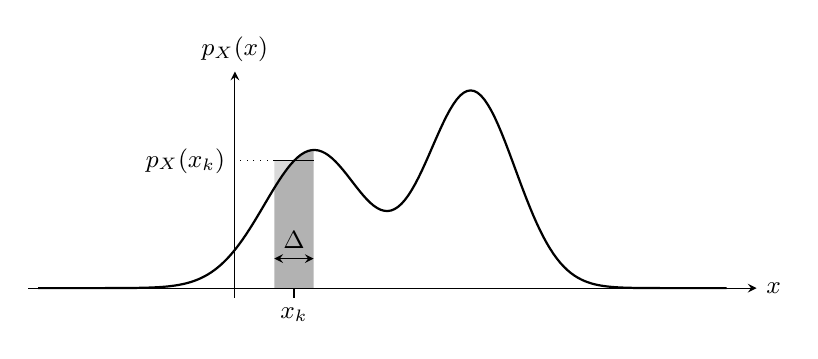
\begin{tikzpicture}
\shorthandoff{>}
%
% Cuantificacion de X
\begin{scope}[xscale=2.5,yscale=2.5]
%
\pgfmathsetmacro{\c}{.4};
\pgfmathsetmacro{\d}{1.2};
\pgfmathsetmacro{\s}{8};
\pgfmathsetmacro{\t}{10};
\pgfmathsetmacro{\a}{.7};
\pgfmathsetmacro{\b}{1};
%
\pgfmathsetmacro{\xk}{.3};
\pgfmathsetmacro{\dx}{.2};
%
% funcion para dibujar una distribucion bimodal (ilustracion de la cuantificacion)
\pgfmathdeclarefunction{bimod}{1}{\pgfmathparse{(\a*exp(-\s*(#1-\c)^2)+\b*exp(-\t*(#1-\d)^2))}}
%
\draw[>=stealth,->] (-1.05,0)--(2.65,0) node[right]{\small $x$};
\draw[>=stealth,->] (0,-.05)--(0,1.1) node[above]{\small $p_X(x)$};
%
% lei de proba
\draw[thick,domain=-1:2.5,samples=200] plot (\x,{bimod(\x)});
%
% dominio alrededor de xk
\fill[domain=\xk-\dx/2:\xk+\dx/2,samples=20,opacity=.3]
({\xk-\dx/2},0)-- plot (\x,{bimod(\x)})--({\xk+\dx/2},0);
%
% xk y Delta
\draw (\xk,0)--(\xk,-.05) node[below]{\small $x_k$};
\draw[>=stealth,<->] ({\xk-\dx/2},.15)--({\xk+\dx/2},.15);
\draw (\xk,.15) node[above]{\small $\Delta$};
%
% recta sobre Delta a altura de p(xk)
\draw ({\xk+\dx/2},{bimod(\xk)})-- ({\xk-\dx/2},{bimod(\xk)});
\draw[dotted] ({\xk-\dx/2},{bimod(\xk)})--(0,{bimod(\xk)})
 node[left]{\small $p_X(x_k)$};
%
% dominio equivalente alrededo de xk
\fill[domain=\xk-\dx/2:\xk,samples=20,opacity=.15]
plot (\x,{bimod(\x)})--({\xk-\dx/2},{bimod(\xk)});
\end{scope}
\end{tikzpicture} \end{center}
%
\leyenda{Densidad  de probabilidad  $p_X$  de $X$,  construcci\'on del  alfabeto
  $\X^\Delta$ donde se define la versi\'on cuantificada $X^\Delta$ de $X$ con su
  distribuci\'on discreta de probabilidad  $p_{X^\Delta}$. La superficie en gris
  oscuro es igual a la superficie definida por el rect\'angulo en gris claro.}
%
\label{Fig:SZ:CuantificacionX}
\end{figure}
%

M\'as  all\'a de esta  notable diferencia  entre la  entrop\'ia y  la entrop\'ia
diferencial, la \'ultima depende de los estados,  es decir que si $Y = g(X)$ con
$g$  biyectiva,  no se  conserva  la  entrop\'ia,  \ie \underline{se  pierde  la
  propiedad~\ref{Prop:SZ:biyeccion}} del caso discreto:
%
\begin{eqnarray*}
H(Y) & = & - \int_{\Rset^d} p_Y(y) \log p_Y(y) \, dy\\[2.5mm]
%
& = &  - \int_{\Rset^d} p_Y(g(x)) \log p_Y(g(x)) \, |\Jac_g(x)| \, dx\\[2.5mm]
%
& = & - \int_{\Rset^d} p_Y(g(x)) \Big( \log \big( p_Y(g(x)) \, |\Jac_g(x)| \big) -
\log |\nabla^t g(x)| \Big) \, |\Jac_g(x)| \, dx
\end{eqnarray*}
%
donde $\Jac_g$ es la matriz Jacobiana
% la  matriz de componentes $\frac{\partial g_i}{\partial x_j}$,
%Jacobiano  
de  la  transformaci\'on  \   $g:  \Rset^d  \mapsto  \Rset^d$  \  
%($g
%\equiv [ g_1(x_1 , \ldots  , x_d) \quad  \cdots \quad g_d(x_1 ,  \ldots ,
%  x_d) ]^t$)
\ y  \ $|\cdot|$  representa el  valor absoluto del  determinante de  la matriz.
Recordando      que     $p_X(x)      =      p_Y(g(x))     |\Jac_g(x)|$      (ver
subsecci\'on~\ref{Ssec:MP:Transformacion},
pagina~\pageref{Ssec:MP:Transformacion}), se obtiene la propiedad siguiente:
%
\begin{propiedadesC}\setcounter{enumi}{\value{PropBiyeccion}}
%
\item\label{Prop:SZ:biyeccionC}
Para  cualquiera biyecci\'on $g:  \Rset^d \mapsto  \Rset^d$
  %
  \[
  H(g(X)) = H(X) + \int_{\Rset^d} p_X(x) \log |\Jac_g(x)| \, dx,
  \]
  %
  donde el \'ultimo t\'ermino, $\Esp\left[  \log |\Jac_g(X)| \right]$ no vale cero
  en general.  En particular, si $H$ es invariante bajo una translaci\'on,
  %
  \[
  H(X+b) = H(X) \quad \forall \: b \in \Rset^d,
  \]
  %
  no  es invariante  por cambio  de escala,
  %
  \[
  H(a X) = H(X) + \log |a| \quad \forall \: a \in \Rset^*.
  \]
\end{propiedadesC}
%
Esta \'ultima  relaci\'on queda v\'alido  para $a$ matriz invertible.   Por esta
\'ultima  relaci\'on, se puede  ver que,  dado $X$,  cuando $a$  tiende a  0, la
entrop\'ia de $a X$ tiende a  $-\infty$.  Es decir que, para $a$ suficientemente
peque\~no,  se  puede  tener $H(a  X)  <  0$,  as\'i que  \underline{se  pierde}
tambi\'en   \underline{la   positividad~\ref{Prop:SZ:positividad}}.   Por   esta
perdida, se quita definitivamente la interpretaci\'on de incerteza/informaci\'on
que hubiera podido tener la entrop\'ia diferencial.

A veces, se usa lo que es llamado potencia entr\'opica:
%
\begin{definicion}[Potencia entr\'opica]
\label{Def:SZ:PotenciaEntropica}
%
  Sea $X$ una variable aleatoria $d$-dimensional. La potencia entr\'opica de $X$
  es definida por
  %
  \[
  N(X) = \frac{1}{2 \pi \e} \exp\left( \frac2d H(X) \right).
  \]
\end{definicion}
%
\noindent Por construcci\'on, $N(X) \ge 0$.  Adem\'as, en el caso continuo, $N(a
X+b)  =  |a|^2 N(X)$  (queda  v\'alido para  una  matriz  $a$ invertible):  esta
propiedad puede justificar  la idea de ``potencia''; adem\'as  $N(a X+b)$ tiende
naturalmente a  cero cuando $a$  tiende a cero.   Se recupera as\'i  la noci\'on
informacional a trav\'es  de $N$ en este  contexto ($a X + b$  ``tiende'' a $b$,
variable determinista).

Si se pierde la propiedad de invarianza bajo una biyecci\'on, sorprendentemente,
se conserva la entrop\'ia bajo el equivalente continuo del rearreglo.
%
%\begin{definicion}[Rearreglo sim\'etrico]\label{Def:SZ:rearreglo}
%  Sea $\P \subset \Rset^d$ abierto de  volumen finito $|\P| < +\infty$.  El {\it
%    rearreglo sim\'etrico} $\P^\downarrow$  de $\P$ es la bola  centrada en 0 de
%  mismo volumen que $\P$, \ie
%  %
%  \[
%  \P^\downarrow  = \left\{  x  \in  \Rset^d \,  :  \: \frac{2  \pi^{\frac{d}{2}}
%      |x|^d}{\Gamma\left(\frac{d}{2}\right)} \le |\P| \right\},
%  \]
%  %
%  donde  $|\cdot|$  denota  la   norma  euclideana.   Eso  es  ilustrado  figura
%  Fig.~\ref{Fig:SZ:ensemblerearreglado}-a.\newline  Sea  $p_X$  una densidad  de
%  probabilidad y sea $\P_t = \{ y \, : \: p_X(y) > t \}$ para cualquier $t > 0$,
%  sus conjuntos  de niveles.  La densidad de  probabilidad~\footnote{Se proba de
%    que  esta funci\'on,  positiva por  definici\'on, suma  a 1.   Adem\'as, por
%    construcci\'on,  depende  \'unicamente  de   $|x|$  y  decrece  con  $|x|$.}
%  rearreglada sim\'etrico $p^\downarrow_X$ de $p_X$ es definida por
%  %
%  \[
%  p^\downarrow_X(x)  =  \int_0^{+\infty}  \un_{\P_u^\downarrow}(x) \,  du.
%  \]
%  %
%  (recuerdense de que $\un_A$ es el indicator  del conjunto $A$)
%  % , \ie $\un_A(x) = 1$ si $x \in A$ y cero sino.
%\end{definicion}
%
%Del hecho  de que $\forall \, t  < \tau \: \Leftrightarrow  \: \P_\tau \subseteq
%\P_t  \:  \Leftrightarrow \:  \P_\tau^\downarrow  \subseteq \P_t^\downarrow$  es
%sencillo   ver   que   si   $x   \in  \P_\tau^\downarrow$,   entonces   $x   \in
%\P_t^\downarrow$,  lo que  conduce a  $p_X^\downarrow(x) >  \tau$  y vice-versa.
%M\'as  all\'a, sobre  $\P_{\tau+d\tau}  \backslash \P_\tau$  la funci\'on  $p_X$
%``vale''   $\tau$   \   y   \   sobre   $\P_{\tau+d\tau}^\downarrow   \backslash
%\P_\tau^\downarrow$  la funci\'on $p_X^\downarrow$  ``vale'' tambien  $\tau$, lo
%que  da \  $\displaystyle  \int_{\P_\tau^\downarrow} p_X^\downarrow(x)  \, dx  =
%\int_{\P_\tau} p_X(x)  \, dx$ \  (ver~\cite{LieLos01, WanMad04} para  une prueba
%m\'as  rigurosa).   La representaci\'on  de  la  definici\'on  es conocida  como
%representaci\'on  en  capas  de  pastel  (``layer cake''  en  ingles).   Eso  es
%ilustrado en la figura Fig.~\ref{Fig:SZ:ensemblerearreglado}-b
%  %
%  \begin{figure}[h!]
%  %
%  \begin{center} 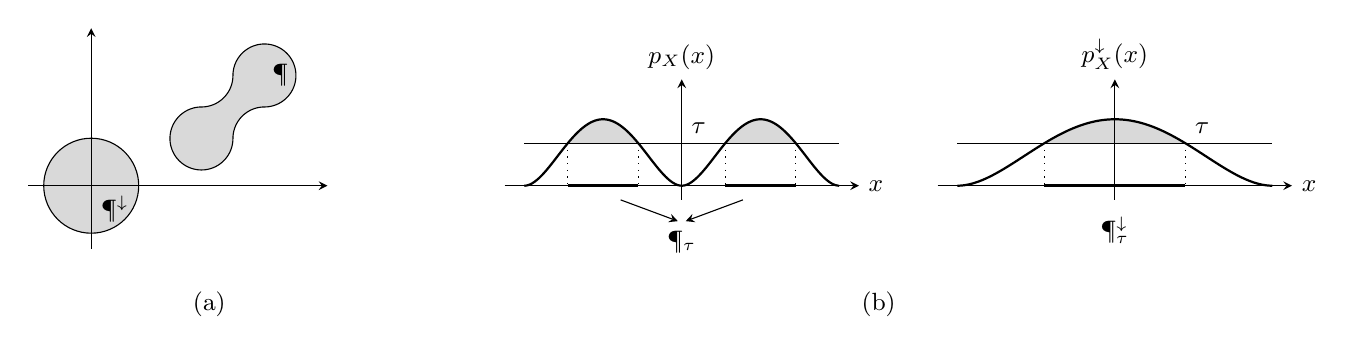
\begin{tikzpicture}
\shorthandoff{>}
%
\begin{scope}[scale=.4]
% Superficia 2*3 pi/4  + 2*2 - 2*pi/4 = 4+pi
\filldraw[draw=black,fill=gray!30]
   plot [domain=0:-270,samples=200] ({cos(\x)+3.5},{sin(\x)+1.5})
-- plot [domain=-90:0,samples=200] ({cos(\x)+3.5},{sin(\x)+3.5})
-- plot [domain=180:-90,samples=200] ({cos(\x)+5.5},{sin(\x)+3.5})
-- plot [domain=90:180,samples=200] ({cos(\x)+5.5},{sin(\x)+1.5})
-- cycle;
\draw (6,3.5) node {\small $\P$};
%
% superficia rearreglada
\filldraw[draw=black,fill=gray!30] (0,0) circle ({sqrt(1+4/pi)});
\draw (.75,-.75) node {\small $\P^\downarrow$};
%
% ejes
\draw[>=stealth,->] (-2,0)--(7.5,0);
\draw[>=stealth,->] (0,-2)--(0,5);
%
\end{scope}
%
%
%----------------------------------------
%
% p_X(x), P_tau...
\begin{scope}[xshift=7.5cm,yscale=1.8]
\pgfmathsetmacro{\t}{.3};
\pgfmathsetmacro{\xt}{sqrt(1-sqrt(32*\t/15))};
\pgfmathsetmacro{\dx}{5.5};% shift para p*(x)
\pgfmathdeclarefunction{studr}{1}{\pgfmathparse{(15/32)*((1-(#1)^2)^2)}}; %Student-r
%
% mezcla de Student-r 15/16 * (1-x^2)^2 (nu = 5) centrados en -1 y 1
% 15/32 (1-(x-a)^2)^2 > t iif (x-a)^2 < 1-sqrt(32*t/15)
% i.e. a-sqrt(1-sqrt(32*t/15)) < x < a+sqrt(1-sqrt(32*t/15))
\fill[domain=-1-\xt:-1+\xt,fill=gray!30] plot(\x,{studr(\x+1)}); % p(x) > tau, x < 0
\fill[domain=1-\xt:1+\xt,fill=gray!30] plot(\x,{studr(\x-1)}); % p(x) > tau, x > 0
\draw[thick,domain=-2:0,samples=100] plot(\x,{studr(\x+1)}); % p(x), x < 0
\draw[thick,domain=0:2,samples=100] plot(\x,{studr(\x-1)}); % p(x), x > 0
\draw (-2,\t)--(2,\t); \draw (0,\t) node[above right]{\small $\tau$}; % y = tau
%
% dominio P_tau
\draw[dotted] ({-1-\xt},{studr(\xt)})--({-1-\xt},0);
\draw[dotted] ({-1+\xt},{studr(\xt)})--({-1+\xt},0);
\draw[very thick] ({-1-\xt},0)--({-1+\xt},0);
\draw[>=stealth,->] ({-1+\xt/2},-.1)--(-.05,-.25);
%
\draw[dotted] ({1-\xt},{studr(\xt)})--({1-\xt},0);
\draw[dotted] ({1+\xt},{studr(\xt)})--({1+\xt},0);
\draw[very thick] ({1-\xt},0)--({1+\xt},0);
\draw[>=stealth,->] ({1-\xt/2},-.1)--(.05,-.25);
%
\draw (0,-.25) node[below]{\small $\P_\tau$};
%
% ejes
\draw[>=stealth,->] (-2.25,0)--(2.25,0) node[right]{\small $x$};
\draw[>=stealth,->] (0,-.1)--(0,.75) node[above]{\small $p_X(x)$};
%
%---------------------------
%
% 15/32 (1-(x-a)^2)^2 > t iif (x-a)^2 < 1-sqrt(32*t/15)
% i.e. a-sqrt(1-sqrt(32*t/15)) < x < a+sqrt(1-sqrt(32*t/15))
% Volumen 2*sqrt(1-sqrt(32*t/15))
% Por simetria, P_t* = [-2*sqrt(1-sqrt(32*t/15)) , 2*sqrt(1-sqrt(32*t/15))]
% da f*(x) = 15/32 (1-x^2/4)^2
\fill[domain=-2*\xt:2*\xt,fill=gray!30] plot({\x+\dx},{studr(.5*\x)}); % p*(x) > tau
\draw[thick,domain=-2:2,samples=200] plot({\x+\dx},{studr(.5*\x)});
\draw ({-2+\dx},\t)--({2+\dx},\t); \draw ({2*\xt+\dx},\t) node[above right]{\small $\tau$}; % y = tau
%
% dominio P_tau*
\draw[dotted] ({-2*\xt+\dx},{studr(\xt)})--({-2*\xt+\dx},0);
\draw[dotted] ({2*\xt+\dx},{studr(\xt)})--({2*\xt+\dx},0);
\draw[very thick] ({-2*\xt+\dx},0)--({2*\xt+\dx},0);
%
\draw (\dx,-.15) node[below]{\small $\P_\tau^\downarrow$};
%
% ejes
\draw[>=stealth,->] ({-2.25+\dx},0)--({2.25+\dx},0) node[right]{\small $x$};
\draw[>=stealth,->] (\dx,-.1)--(\dx,.75) node[above]{\small $p_X^\downarrow(x)$};
\end{scope}
%
\draw (1.5,-1.5) node{\small (a)};
\draw (10,-1.5) node{\small (b)};
\end{tikzpicture} \end{center}
%  %
%  \leyenda{(a):  Ilustraci\'on del rearreglo  sim\'etrico $\P^\downarrow$  de un
%    conjunto  $\P$,  siendo  la  bola  centrada  en 0  de  mismo  volumen.   (b)
%    Construcci\'on  del rearreglo  $p_X^\downarrow$:  dado un  $\tau$, se  busca
%    $\P_\tau$ y  se deduce $P_\tau^\downarrow$; dado  un $x$, se  busca el mayor
%    $t$  tal que  $x  \in  P_t^\downarrow$, este  $t$  m\'aximo siendo  entonces
%    $p_X^\downarrow(x)$; adem\'as,  por construcci\'on, las  superficies en gris
%    son iguales.}
%  %
%  \label{Fig:SZ:ensemblerearreglado}
%  \end{figure}
% =  \B  \left( 0  , r_\P  \right)$ con  $\frac{2
%    \pi^{d/2} r_\P^d}{\Gamma(d/2)} = |\P|$.

\begin{propiedadesC}\setcounter{enumi}{\value{PropPermutacion}}
\item\label{Prop:SZ:permutacionC} {\it invarianza  bajo un rearreglo:} Sea $p_X$
  densidad de probabilidad sobre un abierto de $\Rset^d$,
  %
  \[
  H\left( p_X^\downarrow \right) = H(p_X).
  \]
  donde  $p_X^\downarrow$   es  el  rearreglo  s\'imetrico   de  $p_X$  definido
  Def.~\ref{Def:MP:rearreglo} pagina~\pageref{Def:MP:rearreglo}.
\end{propiedadesC}
%
\noindent Esta  propiedad es probada para  funciones convexas de  la densidad de
probabilidad              por             ejemplo             en~\cite{LieLos01}
o~\cite[Lema~7.2]{WanMad04}~\footnote{En~\cite[Sec.~3.3]{LieLos01}  lo  muestran
  para $\phi(p_X)$  donde $\phi$  es la diferencia  de dos  funciones monotonas,
  siendo $\phi(t)  = t  \log t$ un  caso particular.},  y entonces para  el caso
particular $\phi(t) = t \log t$.

Una pregunta natural  es de saber lo que pasa en  t\'ermino de mayorizaci\'on en
el contexto continuo $d$-dimensional.
% Por  eso, se necesita primero de redefinir
%la noci\'on de mayorizaci\'on en este contexto:
%
%\begin{definicion}[Mayorizaci\'on en el contexto continuo]\label{Def:SZ:MayorizacionC}
%  Una densidad  de probabilidad $p$  es dicha mayorizada por  una distribuci\'on
%  $q$ si:
%  %
%  \[
%  p \prec  q \qquad \mbox{ssi}  \qquad \int_{\B(0,r)} p^\downarrow(x) \,  dx \le
%  \int_{\B(0,r)} q^\downarrow(x) \, dx \quad \forall  \, r > 0, \quad \mbox{ y }
%  \quad \int_{\Rset^d} p^\downarrow(x) \, dx = \int_{\Rset^d} q^\downarrow(x) \,
%  dx,
%  \]
%  %
%  donde \ $\B(0,r) = \{ x \in \Rset^d:  \: \|x\| \ge r \}$ \ es la bola centrada
%  en \ $0$ \ y de rayo  \ $r$ \ (las \'ultimas integrales son obviamente iguales
%  a 1).
%\end{definicion}
%
%\noindent  L
Aparece que la Schur-concavidad~\ref{Prop:SZ:Schurconcavidad}  se conserva  en el
caso  continuo, \ie
%
\[
p \prec  q  \quad \Rightarrow  \quad H(p)  \ge H(q).
\]
%
con      la      relaci\'on      de      mayorizaci\'on      continua      vista
Def.~\ref{Def:MP:MayorizacionC}      pagina~\pageref{Def:MP:MayorizacionC}.       La
desigualdad inversa  es probada  para cualquier funci\'on  $\phi$ convexa  de la
densidad~\cite{Cho74} o~\cite[Prop.~7.3]{WanMad04},  en particular para $\phi(t)
= t \log t$.

Como  se  ha visto,  la  entrop\'ia diferencial  no  es  siempre positiva,  como
consecuencia de la propiedad~\ref{Prop:SZ:biyeccionC}.  Tambi\'en, \underline{la
  propiedad  de cota  superior~\ref{Prop:SZ:cotamaxima} se  pierde}  en general,
\underline{salvo si se ponen v\'inculos}:
%
\begin{propiedadesC}\setcounter{enumi}{\value{PropCotamaxima}}
\item
  \begin{enumerate}
  \item\label{Prop:SZ:cotamaximauniforme} Si $\X$ es de volumen finito $|\X| < +
    \infty$, la entrop\'ia es acotada por arriba,
    %
    \[
    H(X) \le \log |\X|,
    \]
    %
    con igualdad si y solamente si $X$ es \underline{uniforme}.
    %
  \item\label{Prop:SZ:cotamaximagaussiana}  Si  $\X =\Rset^d$  y  $X$ tiene  una
    matriz  de covarianza  dada \  $\Sigma_X =  \Esp\left[ X  X^t \right]  - m_X
    m_X^t$ \ ($m_X = \Esp[X]$), la entrop\'ia es tambi\'en acotada por arriba,
    %
    \[
    H(X) \le \frac{d}{2} \log(2 \pi \e) + \frac12 \log |\Sigma_X|,
    \]
    %
    con igualdad si y solamente si $X$ es \underline{gaussiana}.  En particular,
    la  potencia  entr\'opica de  la  gaussiana  vale  $N(X) =  \left|  \Sigma_X
    \right|^{\frac1d}$, dando de nuevo un  ``sabor'' de potencia a $N$.  Como se
    lo va  a ver en  este cap\'itulo,  la gaussiana juega  un rol central  en la
    teor\'ia de la informaci\'on.
  \end{enumerate}
  En  ambos casos,  estas  desigualdades con  la  distribuci\'on maximizante  se
  obtienen resolviendo el  problema de maximizaci\'on de la  entrop\'ia sujeto a
  v\'inculos.    Se  trata   del   caso  m\'as   general   en  la   subsecci\'on
  Sec.~\ref{Ssec:SZ:MaxEnt}.
\end{propiedadesC}

Al    final,   \underline{se   conservan    obviamente   las    propiedades   de
  concavidad~\ref{Prop:SZ:concavidad},  de aditividad~\ref{Prop:SZ:aditividad} y
  de sub-aditividad~\ref{Prop:SZ:subaditividad}}.   Es interesante notar  que de
la  desigualdad~\ref{Prop:SZ:subaditividad},  puramente  entr\'opica,  se  puede
deducir la  desigualdad de Hadamard,  desigualdad puramente matricial:  $|R| \le
\prod_i R_{i,i}$ para cualquiera  matriz sim\'etrica definida positiva (viene de
la   propiedad~\ref{Prop:SZ:subaditividad}  escrita   para   una  gaussiana   de
covarianza $R$ y tomando una exponencial de la desigualdad).

\

Como lo hemos  visto, la entrop\'ia y su versi\'on diferencial  no tienen ni las
mismas  propiedades, ni  completamente la  misma interpretaci\'on.  Sin embargo,
varias  propiedades  se  comparten y  se  proban  de  la  misma manera.  De  las
escrituras, con una  suma o una integral, a veces se  encuentra en la literatura
la escritura \'unica \ $\sumint$ \ para significar que se usa la suma en el caso
discreto, y la integraci\'on en el caso continuo con densidad~\cite{Rio07}.  Sin
embargo,   volviendo  al   fin   de  la   subsecci\'on~\ref{Ssec:MP:VAContinua},
pagina~\pageref{Pagina:MP:DensidadDiscreta}    \    y    a    la    definici\'on
Def.~\ref{Def:MP:Dirac} de una medida discreta sobre \ $\X = \{ x_j \}_j$ \ dada
por \ $\mu_\X = \sum_j \delta_{x_j}$, vimos de que en el caso discreto \ $p_X$ \
es la densidad de la medida de probabilidad con respeto a \ $\mu_\X$.  Adem\'as,
de  la propiedad  $\displaystyle \int_\Rset  f(x) \  d\delta_{x_j} =  f(x_j)$ se
puede ver  una suma  como una integral  con respeto  a une medida  discreta.  De
estas observacione, se puede escribir de la misma forma la entrop\'ia discreta y
diferencial:
%
\begin{definicion}[Escritura \'unica de la entrop\'ia]
\label{Def:SZ:ShanonMu}
%
  Sea  \  $X$  \  variable  aleatoria definida  sobre  $\X  \subseteq  \Rset^d$,
  admitiendo una densidad  de probabilidad \ $p_X$ \ con respeto  a una medida \
  $\mu$ \  (ej. $\mu_\X$  \ en el  caso discreto \  $\mu =  \mu_L$ \ en  el caso
  diferencial). La entrop\'ia de $X$  \underline{con respeto a $\mu$} se escribe
  como
  %
  \[
  H(X) \equiv H(p_X) = - \int_\X p_X(x) \, \log(p_X) \, d\mu(x)
  \]
  %
  Insistamos  en  el hecho  de  que se  puede  entender  esta definici\'on  para
  cualquier $\mu$ y densidad con respeto a $\mu$, que sea discreta, de Lebesgue,
  o cualquiera.
\end{definicion}